\documentclass{IEEEtran}
\usepackage[utf8]{inputenc}
\usepackage{cite}
\usepackage{amsmath}
\usepackage{amsfonts}
\usepackage{amssymb}
\usepackage{float}
\newcommand\norm[1]{\left\lVert#1\right\rVert}
\usepackage[flushleft]{threeparttable}
\usepackage[urlcolor=black,linkcolor=black,citecolor=black,colorlinks=true]{hyperref}
\usepackage{graphicx}
\newcommand\bmat[1]{\begin{bmatrix}#1\end{bmatrix}}
\newcommand{\mat}[1]{\boldsymbol{#1}}

\title{Left-Invariant EKF for Robot Localization:\\%
A Mobile Robotics Project}
\author{}
%
\begin{document}
\maketitle

\begin{abstract}
In this project we derive and implement a Left-Invariant Extended Kalman Filter (LI-EKF) for quadrotor localization in MATLAB and C++. We applied our filter to simulated data that we generated and also to the Zurich Urban Micro Aerial Vehicle Dataset Dataset \cite{majdik2017zurich}. The filter takes in IMU data for prediction and GPS data for correction. A traditional EKF is implemented as a baseline for comparison. For the simulated data, the tracking of the left-invariant EKF is accurate and has outperformed that of the tradition EKF in both orientation and position. It also achieved decent tracking result with Zurich Urban Dataset, though the estimation is highly dependent on GPS.
\end{abstract}

\section{Introduction}
The process model of a 6 degree of freedom vehicle is nonlinear, and there is no general method to design a globally stable observer.  Historically, methods have relied on linearizing the process model by using first order approximations (EKF) or performing an unscented transform (UKF)\cite{thrun2005probabilistic}.  These methods are practical for applications that operate in a small region where linear approximations are valid, but for aerial vehicles undergoing large rotations there is a limited envelope for which they are effective.  Therefore, in order to provide an accurate state estimation over the full flight envelope, we seek an observe that is capable of handling such maneuvers without relying on the traditional techniques. 

For nonlinear process that are group affine, it is possible to design an invariant observer with guaranteed global convergence\cite{InEKF_Barrau}. In this paper, we present an Invariant EKF that uses an inertial measurement unit (IMU) and a gyroscope for prediction and GPS for an update. This filter measures the full state of the rigid body, including the position, velocity, and orientation. The filter is tested using simulated data we generated and the Zurich Urban Dataset.

%\section{Theoretical Background}
%%%% Do we need to put the definition here? Feels it might be the same as Manni's paper.
\textbf{Definition}: the right- and left-invariant errors between two trajectories $\textbf{X}_t$ and $\tilde{\textbf{X}}_t$ are:
\begin{align*}
    & \mathbf{\eta}^r_t = \hat{\textbf{X}}_t\textbf{X}_t^{-1} = (\hat{\textbf{X}}_t\textbf{L})(\textbf{X}_t\textbf{L})^{-1}
    & (right-invariant) \\
    & \mathbf{\eta}^l_t = \textbf{X}_t^{-1}\hat{\textbf{X}_t} = (\textbf{L}\hat{\textbf{X}}_t)^{-1}(\textbf{L}\textbf{X}_t)
    & (right-invariant)
\end{align*}
% brief introduction of InEKF and theorems

\section{bias-corrected Left-Invariant EKF}
%%%%%%%%%%%%%%%%%%%%%%%%%%%%%%%%%%%
\subsection{State Representation in $SE_2(3)$}
Our goal is to track the robots orientation, velocity, and position over time. We define this state and the estimation error in $SE_2(3)$ because the error dynamics have the properties of logarithm-linearity and autonomy. Thus, the state variable $\mathbf{X}_t$, containing the orientation $\mathbf{R}(t)$, velocity $\mathbf{v}(t)$ in body frame, and the position $\mathbf{p}(t)$ in world frame, is defined as:
\begin{gather*}
    \mathbf{X}_t =
    \begin{bmatrix}
        \mathbf{R}(t) & \mathbf{v}(t) & \mathbf{p}(t) \\
        \mathbf{0}_{1 \times 3} & 1 & 0 \\
        \mathbf{0}_{1 \times 3} & 0 & 1
    \end{bmatrix}
\end{gather*}

%%%%%%%%%%%%%%%%%%%%%%%%%%%%%%%%%%%
\subsection{IMU and Gyro System Dynamics}
Firstly, without taking IMU bias into account, we only add a white Gaussian noise:
\begin{align}
    & \tilde{\mat{\omega}}_t = \mat{\omega}_t + \mat{w}^g_t 
    & \mat{w}^g_t \sim \mathcal{GP}(\mat{0}_{3,1},\Sigma^g)\\
    & \tilde{\mat{a}}_t = \mat{a}_t + \mat{w}^a_t
    & \mat{w}^a_t \sim \mathcal{GP}(\mat{0}_{3,1},\Sigma^a)
\end{align}
where $\tilde{\mat{\omega}}_t$ and $\tilde{\mat{a}}_t$ are the measured angular velocity from the gyroscope and measured linear acceleration from the accelerometer.

Using IMU measurements, the continuous-time system dynamics can be represented as:
\begin{align}
    & \frac{d}{dt}\mat{R}_t = \mat{R}_t[\tilde{\mat{\omega}}_t - \mat{w}^g_t]_\times \label{eqn:rot_dyn}\\
    & \frac{d}{dt}\mat{v}_t = \mat{R}_t(\tilde{\mat{a}}_t-\mat{w}^a_t) + \mat{g} \label{eqn:vel_dyn}\\
    & \frac{d}{dt}\mat{p}_t = \mat{v}_t \label{eqn:pos_dyn}
\end{align}
%could be deleted if no room~~~~~~~~~
Collecting terms in matrix form and writing the process model with respect to current state $X_t$ yields:
\begin{multline}
    \frac{d}{dt}\mat{X}_t =
    \begin{bmatrix}
        \mat{R}_t[\tilde{\mat{\omega}_t}]_\times & \mat{R}_t\tilde{\mat{a}_t} + g & \mat{v}_t \\
        \mat{0}_{1 \times 3} & 0 & 0 \\
        \mat{0}_{1 \times 3} & 0 & 0
    \end{bmatrix}
    - \\
    \begin{bmatrix}
        \mat{R}_t & \mat{v}_t & \mat{p}_t \\
        \mat{0}_{1 \times 3} & 1 & 0 \\
        \mat{0}_{1 \times 3} & 0 & 1 
    \end{bmatrix}
    \begin{bmatrix}
        [\mat{w}^g_t]_\times & \mat{w}^a_t & \mat{0}_{3,1} \\
        \mat{0}_{1 \times 3} & 0 & 0 \\
        \mat{0}_{1 \times 3} & 0 & 0
    \end{bmatrix}\\
     = f_{u_t}(\mat{X}_t) - \mat{X}_t\mat{w}_t^\wedge
\end{multline}
where $\mat{w}_t \triangleq [\mat{w}^g_t, \mat{w}^a_t, \mat{0}_{1x3}]^T$.
%could be deleted if no room~~~~~~~~~

For the hybrid robot estimation problem with continuous-time motion model and discrete-time observation model, we discretized the above continuous-time system dynamics Eqns.~(\ref{eqn:rot_dyn}, \ref{eqn:vel_dyn}, \ref{eqn:pos_dyn}). With the assumption that the angular velocity and the linear acceleration remain unchanged over a short period $\Delta t$, we can write the discrete process model from step $k$ to $k+1$ as the following:
\begin{align}
    & \mat{R}_{k+1} = \mat{R}_k \mat{\Gamma}_0 (\mat{\omega}_k \Delta t) \\
    & \mat{v}_{k+1} = \mat{v}_k + \mat{R}_k \mat{\Gamma}_1 (\mat{\omega}_k \Delta t) \mat{a}_k \Delta t + \mat{g} \Delta t \\
    & \mat{p}_{k+1} = \mat{p}_k + \mat{v}_k \Delta t + \mat{R}_k \mat{\Gamma}_2 (\mat{\omega}_k \Delta t) \mat{a}_k \Delta t^2 + \frac{1}{2}\mat{g} \Delta t^2
\end{align}
%\tilde{\mat{\omega}}_t = \mat{\omega}_t + \mat{w}^g_t 
where $\mat{\omega}_k = \tilde{\mat{\omega}}_k-\mat{w}^g_k$ and $\mat{a}_k = \tilde{\mat{a}}_k-\mat{w}^a_k$. $\mat{w}^g_k$ and $\mat{w}^a_k$ are the white noise of motion model for the angular velocity and linear acceleration respectively. The derivation of $\Gamma_i$ functions are explained in detail in Appendix \ref{sec:dyn_sec} and used here to get the state transition matrices:
%could be deleted if no room~~~~~~~~~
\begin{align}
    & \mat{\Gamma}_0(\phi) = \mat{I}_3 + \frac{\sin(\norm{\mat{\phi}})}{\norm{\mat{\phi}}}[\mat{\phi}]_\times 
    + \frac{1-\cos(\norm{\mat{\phi}})}{\norm{\mat{\phi}}^2}[\mat{\phi}]^2_\times \\
    & \mat{\Gamma}_1(\mat{\phi}) = \mat{I}_3 + \frac{1-\cos(\norm{\mat{\phi}})}{\norm{\mat{\phi}}^2}[\mat{\phi}]_\times\nonumber\\
    & \quad\quad\quad\quad\quad\quad\quad\quad\quad\quad\quad\quad
    + \frac{\norm{\mat{\phi}}-\sin(\norm{\mat{\phi}})}{\norm{\mat{\phi}}^3}[\phi]^2_\times \\
    & \mat{\Gamma}_2(\mat{\phi}) = \frac{1}{2}\mat{I}_3 + \frac{\norm{\mat{\phi}}-\sin(\norm{\mat{\phi}})}{\norm{\mat{\phi}}^3}[\mat{\phi}]_\times\nonumber\\
    & \quad\quad\quad\quad\quad\quad\quad\quad\quad +\frac{\norm{\mat{\phi}}^2+2\cos(\norm{\mat{\phi}})-2}{2\norm{\mat{\phi}}^4}[\mat{\phi}]^2_\times
\end{align}
Where $\mat{\Gamma}_0(\mat{\phi})$ is the exponential map of SO(3), and $\mat{\Gamma}_1(\mat{\phi})$ is the left Jacobian of SO(3).
%could be deleted if no room~~~~~~~~~

%%%%%%%%%%%%%%%%%%%%%%%%%%%%%%%%%%%
\subsection{Error Dynamics}

With measurements coming from GPS in global frame, We choose the left invariant error $\mathbf{\eta}^l_t$:
\begin{align*}
    & \mat{\eta}^l_t = \textbf{X}_t^{-1}\Bar{\textbf{X}_t} = (\textbf{L}\Bar{\textbf{X}_t})^{-1}(\textbf{L}\textbf{X}_t)
\end{align*}
With Lie group action, we get corresponding error in Lie algebra:
%eqns1
\begin{align}
    & \mat{\eta}^l_t = \exp([\mat{\xi}^l_t]_{\times})
\end{align}
where $\exp([\mat{\xi}^l_t]_{\times})\approx I + [\mat{\xi}^l_t]_{\times}$, and the $\approx$ should be $=$ from the logarithm-linear property of error in Lie group.

The skew operator $[\cdot]_\times$ :  $\mathbb{R}^9 \rightarrow \mathfrak{se}_2(3)$ is a mapping from vector basis to Lie algebra matrix basis. It is defined as:
\begin{equation}
    [\mat{\xi}]_\times = 
    \begin{bmatrix}
    [\mat{\xi}^R]_\times & \mat{\xi}^v & \mat{\xi}^p \\
    \mat{0}_{1 \times 3} & 0 & 0 \\
    \mat{0}_{1 \times 3} & 0 & 0 \\
    \end{bmatrix}
\end{equation}
Where the $[\mat{a}]_\times$ operator for $\mat{\xi}^R$ denotes the transformation $\mathbb{R}^3 \rightarrow so(3)$:
\begin{equation}
    \mat{a} =  
    \begin{bmatrix}
        a_1 \\ a_2 \\ a_3 
    \end{bmatrix} \implies
    [\mat{a}]_\times = 
    \begin{bmatrix}
        0 & -a_3 & a_2 \\
        a_3 & 0 & -a_1 \\
        -a_2 & a_1 & 0 \\
    \end{bmatrix}
\end{equation}

In order to find the error dynamics equation in Lie algebra as the following form with $\mat{w}_t$ as the motion noise and its covariance defined as $\mat{Q}_t$:
\begin{align}
    & \frac{d}{dt}[\mat{\xi}^l_t]_{\times}  = A^l_t[\mat{\xi}^l_t]_{\times} + \mat{w_t}
\end{align}
we substitute the above elegant linear equation into system dynamics equations and obtain the error Jacobian matrix $\mat{A}_t$:
\begin{align}
    & \mat{A}^l_t = 
    \begin{bmatrix}
    -[\hat{\mat{\omega}_t}]_\times & \mat{0} & \mat{0} \\
    -[\hat{\mat{a}}_t]_\times & -[\hat{\mat{\omega}}_t]_\times & \mat{0} \\
    \mat{0} & \mat{I}_{3 \times 3} & -[\hat{\mat{\omega}}_t]_\times \\
    \end{bmatrix} 
\end{align}

Therefore the covariance of the left invariant error could be computed through Riccati equation:
\begin{equation}
    \frac{d}{dt}\mat{P}_t=\mat{A}_t\mat{P}_t+\mat{P}_t\mat{A}_t^T+\mat{Q}_t
\end{equation}

%While the inverse operation would be wedge operator $(\cdot)^\vee : \mathfrak{g} \rightarrow \mathbb{R}^9$, defined by:
%\begin{equation}
%    Ad_{\mat{X}_t} = 
%    \begin{bmatrix}
%        \mat{R} & \mat{0} & \mat{0} \\
%        (\mat{v}_t)_\times\mat{R}_t & \mat{R}_t & \mat{0} \\
%        (\mat{p}_t)_\times\mat{R}_t & \mat{0} & \mat{R}_t
%    \end{bmatrix}
%\end{equation}


%%%%%%%%%%%%%%%%%%%%%%%%%%%%%%%%%%%
\subsection{Left-invariant observation model}
In order to get a invariant observation model in Lie group, we rearrange every measurement from GPS as:
%eqns2
\begin{align}
    & \textbf{Y}_k = \textbf{X}_k \mat{b} + \textbf{V}_k \\
    & \begin{bmatrix}
        x_{gps} \\ y_{gps} \\ z_{gps} \\ 0 \\ 1
      \end{bmatrix} =
      \begin{bmatrix}
        \mat{R}_k & \mat{v}_k & \mat{p}_k \\
        \mat{0} & 1 & 0 \\
        \mat{0} & 0 & 1 \\
      \end{bmatrix}
      \begin{bmatrix}
        0 \\ 0 \\ 0\\ 0 \\ 1
      \end{bmatrix} +
      \begin{bmatrix}
        \mat{q}_k \\ 0 \\ 0
      \end{bmatrix}
\end{align}
where $\mat{q}_k$ is measurement white noise with covariance $\mat{\Sigma}^q$.

To fit in the Kalman filter correction model, we calculate the Jacobian H by:
\begin{multline}
    \mat{H}\mat{\xi^r_t} = \mat{\xi^r_t} \mat{b} = 
    \begin{bmatrix}
       \mat{\xi^R_t} & \mat{\xi^{v}_t} & \mat{\xi^{p}_t}  \\
       \mat{0}       & 0         & 0 \\
       \mat{0}       & 0         & 0
    \end{bmatrix}
    \begin{bmatrix}
        \mat{0} \\
        0 \\
        1
    \end{bmatrix}\\
    =
    \begin{bmatrix}
        \mat{0}_{3 \times 3} & \mat{0}_{3 \times 3} & \mat{I}_{3 \times 3} \\
        \mat{0}_{1 \times 3} & \mat{0}_{1 \times 3} & \mat{0}_{1 \times 3} \\
        \mat{0}_{1 \times 3} & \mat{0}_{1 \times 3} & \mat{0}_{1 \times 3} 
    \end{bmatrix}
    \begin{bmatrix}
         \mat{\xi^R_t} \\
         \mat{\xi^v_t} \\
         \mat{\xi^p_t}
    \end{bmatrix}
\end{multline}

Considering computational efficiency, we choose H in its reduced form (Eq. \ref{eqn:H}) and the corresponding compensation is made later when calculating the Kalman gain.
\begin{equation}
    \label{eqn:H}
    \mat{H} = 
    \begin{bmatrix}
    \mat{0} & \mat{0} & \mat{I}_{3 \times 3}
    \end{bmatrix}
\end{equation}

In the correction step, an innovation vector is found to quantify new information:  
%eqns3
\begin{align}
    \mat{\nu}_k = \bar{\mat{X}}^{-1}_k \mat{Y}_k - b
\end{align}

After substituting the relationship between state and error in Lie algebra, we got the covariance of innovation as:
\begin{equation}
    \mat{S}_k=\mat{H}_k\bar{\mat{P}}_k\mat{H}_k^T+\bar{\mat{N}}_k
\end{equation}
where $\bar{\mat{N}}_k$ is the reduced form of $\mat{N}_k$:
\begin{align}
    & \mat{N}_k=\bar{\mat{X}}_k^{-1}
    \begin{bmatrix}
    \mat{\Sigma}^{q} & & \\
    & \mat{0} & \\
    & & \mat{0} \\
    \end{bmatrix} 
    \bar{\mat{X}}_k\\
    & \bar{\mat{N}}_k=\bar{\mat{R}}_k^T\mat{\Sigma}^q\bar{\mat{R}}_k
\end{align}

%%%%%%%%%%%%%%%%%%%%%%%%%%%%%%%%%%%%%%%%
\subsection{Including IMU Biases}
In actual application, IMU usually has biases which corrupt the measurements progressively. Hence we modify the input of IMU system dynamics model as below:
\begin{align}
    & \tilde{\mat{\omega}}_t = \mat{\omega}_t + \mat{b}^g_t + \mat{w}^g_t 
    & \mat{w}^g_t \sim \mathcal{GP}(\mat{0}_{3,1},\Sigma^g) \\
    & \tilde{\mat{a}}_t = \mat{a}_t + \mat{b}^a_t + \mat{w}^a_t
    & \mat{w}^a_t \sim \mathcal{GP}(\mat{0}_{3,1},\Sigma^a)
\end{align}

Since each bias term remains almost unchanged between every time step, we choose the Brownian motion model for bias dynamics: 
\begin{align}
    & \frac{d}{dt}\mat{b}^g_t = \mat{w}^{bg}_t 
    & \mat{w}^{bg}_t \sim \mathcal{GP}(\mat{0}_{3,1},\Sigma^{bg}) \\
    & \frac{d}{dt}\mat{b}^a_t = \mat{w}^{ba}_t
    & \mat{w}^{ba}_t \sim \mathcal{GP}(\mat{0}_{3,1},\Sigma^{ba})
\end{align}

We combine all biases in a single vector (Eq. \ref{eqn:bias}), and augment the error vector with the error in lie algebra (Eq. \ref{eqn:bias_aug}) instead of the state directly to avoid dimensional inconsistency. Then we found the new error Jacobian matrix $\mat{A}^l_t$, and compared the result with that in the paper of Hartley \cite{hartley2020iekf}.
\begin{align}
    &  \mat{\theta}_k \triangleq 
        \begin{bmatrix}
            b^g_t \\ b^a_t
        \end{bmatrix}
        \in \mathbb{R}^6
    &\label{eqn:bias}\\
    & \frac{d}{dt}\bmat{\mat{\xi}_t\\\mat{\zeta}_t}=\mat{A}_t\bmat{\mat{\xi}_t\\\mat{\zeta}_t} + \mat{w}_t
    &\label{eqn:bias_aug}\\
    & \mat{A}^l_t = 
    \begin{bmatrix}
    -[\hat{\mat{\omega}_t}]_\times & \mat{0} & \mat{0} & -\mat{I}_{3 \times 3} & \mat{0} & \\
    -[\hat{\mat{a}}_t]_\times & -[\hat{\mat{\omega}}_t]_\times & \mat{0} & \mat{0} & -\mat{I}_{3 \times 3} \\
    \mat{0} & \mat{I}_{3 \times 3} & -[\hat{\mat{\omega}}_t]_\times & \mat{0} & \mat{0} \\
    \mat{0} & \mat{0} & \mat{0} & \mat{0} & \mat{0} \\
    \mat{0} & \mat{0} & \mat{0} & \mat{0} & \mat{0}
    \end{bmatrix}
\end{align}
where $\mat{w}_t \triangleq [\mat{w}^g_t, \mat{w}^a_t, \mat{0}_{1 \times 3}, \mat{w}^{bg}_t, \mat{w}^{ba}_t]^T$ and its covariance is defined as $\mat{Q}_t$

With the bias term corrected, the system dynamics and the prediction model now become:
\begin{align}
    & \bar{\mat{R}}_{k+1} = \mat{R}_{k} \mat{\Gamma}_0 (\bar{\mat{\omega}}_k \Delta t) \\
    & \bar{\mat{v}}_{k+1} = \mat{v}_k + \mat{R}_{k} \mat{\Gamma}_1 (\bar{\mat{\omega}}_k \Delta t) \bar{\mat{a}}_k \Delta t + \mat{g} \Delta t \\
    & \bar{\mat{p}}_{k+1} = \mat{p}_k + \mat{v}_k \Delta t + \mat{R}_{k} \mat{\Gamma}_2 (\bar{\mat{\omega}}_k \Delta t) \bar{\mat{a}}_k \Delta t^2 + \frac{1}{2}\mat{g} \Delta t^2\\
    &\bar{\mat{\theta}}_k = \mat{\theta}_{k-1}\\
    & \bar{\mat{P}}_k=\mat{\Phi}_k\mat{P}_{k-1}\mat{\Phi}_k^T + \mat{\Phi}_k\mat{Q}_{t}\mat{\Phi}_k^T\Delta t
\end{align}
where $\mat{\Phi}_k=\exp(\mat{A}_t\Delta t)$ is the state transition matrix, $\bar{\mat{\omega}}_k = \tilde{\mat{\omega}}_k-\mat{w}^g_k$ and $\bar{\mat{a}}_k = \tilde{\mat{a}}_k-\mat{w}^a_k$ are the bias-corrected input, $\mat{w}^g_k$ and $\mat{w}^a_k$ are the bias terms for the angular velocity and linear acceleration respectively.

After biases appended, we manually add two zero components to the Jacobian H to account for the bias term and update them simultaneously with the state by partitioning the Kalman gain in two parts:
\begin{align}
    & \mat{H}_t = 
    \begin{bmatrix}
        \mat{0} & \mat{0} & \mat{I}_{3 \times 3} & \mat{0} & \mat{0}
    \end{bmatrix}\\
    &     \mat{S}_k=\mat{H}_k\bar{\mat{P}}_k\mat{H}_k^T+\bar{\mat{N}}_k\\
    & \mat{K}_k=\bmat{\mat{K}_k^\xi\\\mat{K}_k^\zeta}=\bar{\mat{P}}_k\mat{H}_k^T\mat{S}_k^{-1}
\end{align}

Then the final bias-corrected correction model is:
\begin{align}
    \mat{X}_k&=\bar{\mat{X}}_k\exp[\mat{K}_k^\xi\Pi(\bar{\mat{X}}_k^{-1}\mat{Y}_k)]\\
    \mat{\theta}_k&=\bar{\mat{\theta}_k}+\mat{K}_k^\zeta\Pi(\bar{\mat{X}}_k^{-1}\mat{Y}_k)\\
    \mat{P}_k&=(\mat{I}-\mat{K}_k\mat{H}_k)\bar{\mat{P}_k}(\mat{I}-\mat{K}_k\mat{H}_k)^T+\mat{K}_k\bar{\mat{N}_k}\mat{K}_k^T
\end{align}
where $\mat{\Pi} = [\mat{I}_{3 \times 3},  \mat{0}_{3 \times 2}]$ is a constant matrix to eliminate effects from truncating zero rows in $\mat{H}$.

What also should be noted here is the estimated covariance is in the Lie algebra, and we need to transfer it to the Cartesian space to plot the uncertainty, for which one way is to use the unscented transform and get the covariance in Cartesian space by propagating the corresponded vector in Lie algebra of estimated state.


\section{Simulation Results} \label{sec:simulation_results}
%%%%%%%%%%%%%%%%%%%%%%%%%%%%%%%%%%%%%%%%
\subsection{Data Preprocessing}
The LI-EKF is tested with two types of data, i.e., simulated data generated by the group and Zurich Urban Micro Aerial Vehicle Dataset \cite{majdik2017zurich}. 

Onboard Pose data from PX4 autopilot board and onboard GPS data are utilized. GPS data is in international WGS 84 (GPS) coordinate system, which are transformed into world frame and aligned with pose coordination system. The noise covariance matrix of the GPS is calculated by taking the covariant of error between GPS and the ground truth data included in the Dataset. 

%%%%%%%%%%%%%%%%%%%%%%%%%%%%%%%%%%%%%%%%
\subsection{Verification with Simulated Data}

We ran a series of tests using a generated set of data to test the accuracy of the filter and test its robustness to input noise.  The set of tests was run on the MATLAB version of the filter in order to use the built in plotting feature to provide a visual verification.  We also used the simulated data tests to generate test cases for the C++ version of the filter, which are added as additional tests in its testing suite.

The simulated data consists of a set of state variables and their derivatives, created from a set of random polynomials which are functions of time.  First, we generate six polynomials, three for the position $(x, y, z)$ in the world frame and three for the angle axis rotation of the body frame with respect to the world frame.  From the position polynomials, we take the derivative once to get the velocity as a function of time and once more to get the acceleration.  Using the time data input as a parameter, we sample the polynomials at the desired time points and save the data.  We similarly generate rotation matrices from the angle axis polynomials for each time point, and take the discrete derivative between time points to find the angular rates.  The world frame acceleration is then rotated into the body frame, after having the gravity bias that an accelerometer would measure added to it.  At the end of the procedure, we provide ourselves with simulated IMU measurements along with the exact ground truth data from which it was generated.

While simulation on "perfect" simulated data can be a good first check for the filter, we also verify the filter after corrupting the simulated data with random noise.  In order to more closely simulate the measurements obtained by a real IMU, we add zero mean Gaussian noise to the angular rate and body frame acceleration measurements. The noise has a tunable covariance parameter to achieve the desired noise level.

% polynomials seeded with rng(2)
\begin{figure}
    \centering
    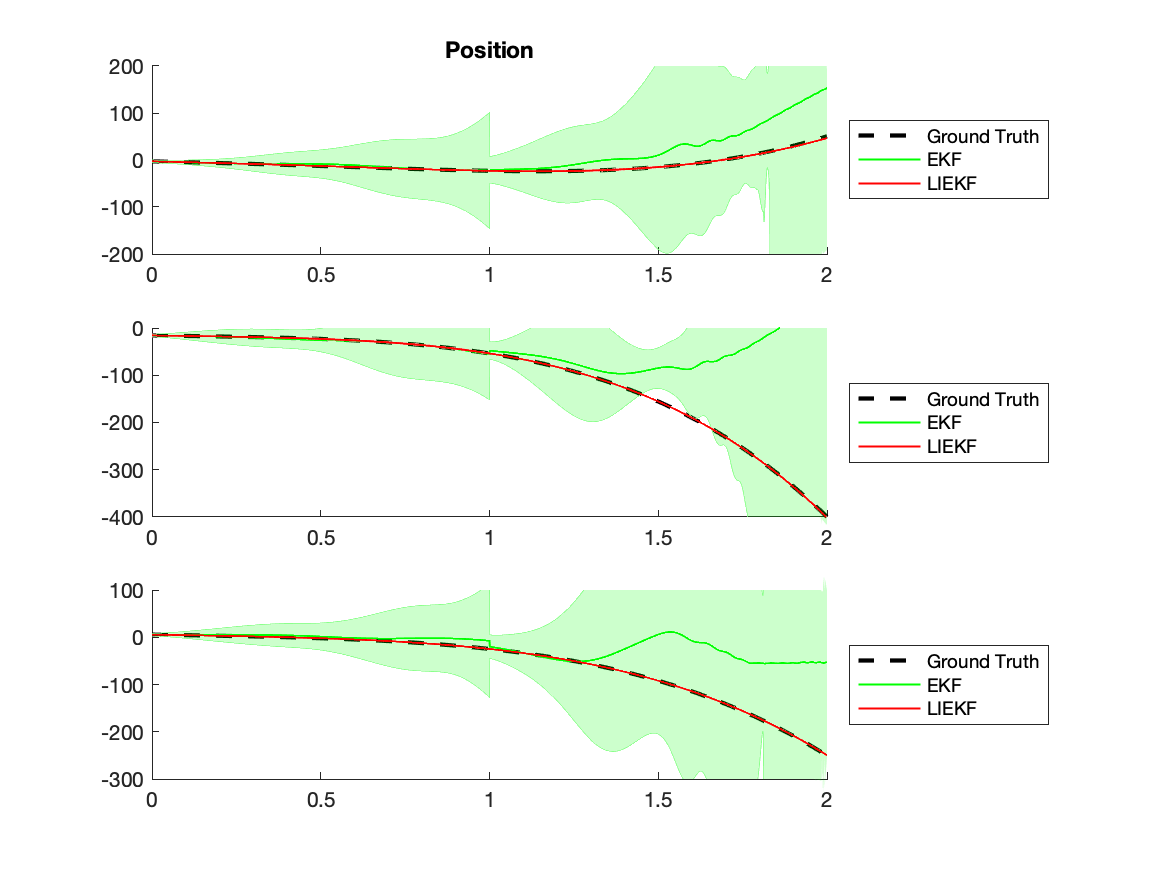
\includegraphics[width=0.45\textwidth]{sections/figures/fake_data_position_nonoise.png}
    \caption{(Simulated data, measurements without noise) EKF (solid green) and LIEKF (solid red) closely follow and converge to the ground truth (dashed black) from perturbed initial conditions. The covariance of each filter is shown as the shaded zone}
    \label{fig:fake_data_pos}
\end{figure}

\begin{figure}
    \centering
    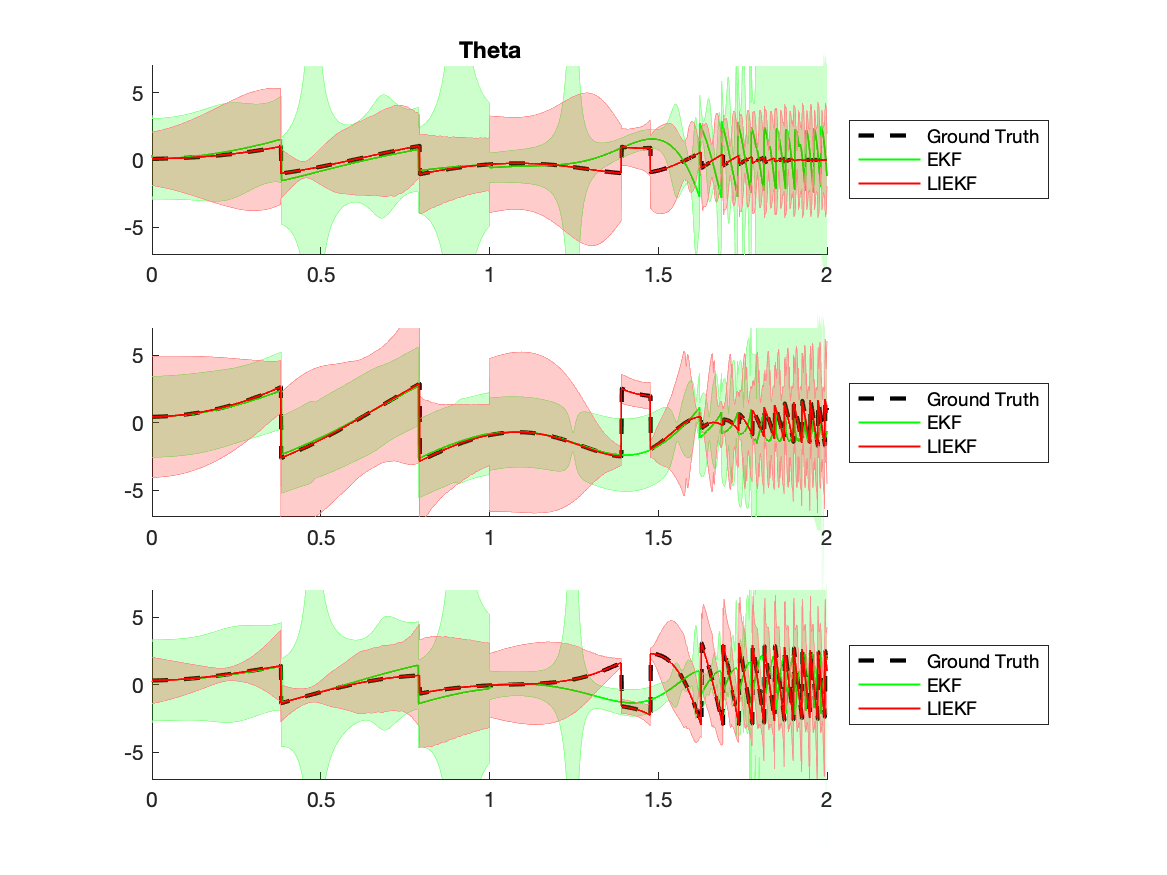
\includegraphics[width=0.45\textwidth]{sections/figures/fake_data_theta_nonoise.png}
    \caption{(Simulated data, measurements without noise) EKF (solid green) and LIEKF (solid red) closely follow and converge to the rotational state of the body. Quantity plotted is $\theta = \mathrm{Log}(R)$, where $R$ is the rotation of the body. The covariance of each filter is shown as the shaded zone}
    \label{fig:fake_data_ang}
\end{figure}

The plots in Figs.~(\ref{fig:fake_data_pos}, \ref{fig:fake_data_ang}) show a simulated run on the filter with no noise, but with position initial conditions perturbed from the ground truth.  The polynomial functions used for the position and angle are listed in Appendix (\ref{sec:fake_data}).  The plots show that the filter converges in both the position and the orientation, and continues to follow the ground truth after converging. The variance of estimation from LI-EKF is bounded well along the trajectory, demonstrating the benefits of autonomous error dynamics.

\begin{figure}
    \centering
    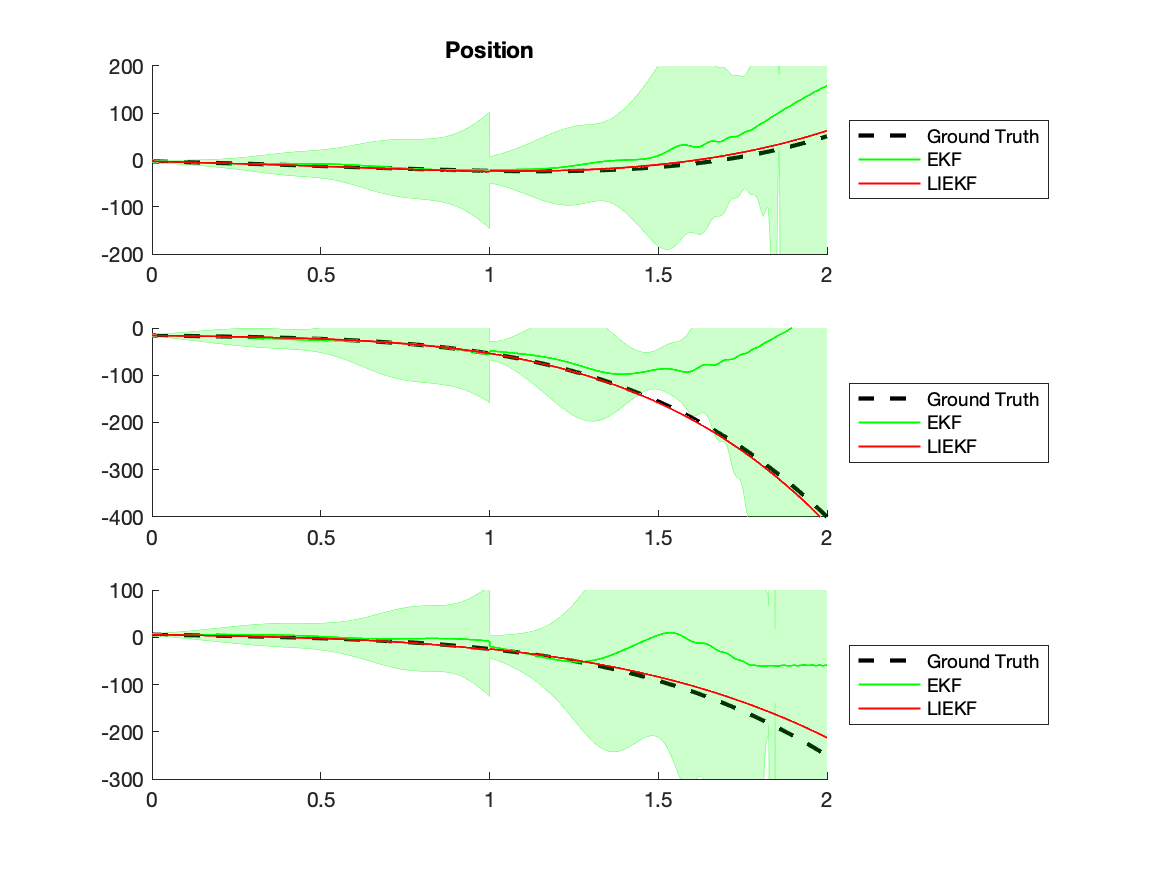
\includegraphics[width=0.45\textwidth]{sections/figures/fake_data_position_noise.png}
    \caption{(Simulated data, measurements with noise) EKF (solid green) and LIEKF (solid red) closely follows ground truth position despite noisy accelerometer reading. The covariance of each filter is shown as the shaded zone}
    \label{fig:fake_data_pos_noise}
\end{figure}

\begin{figure}
    \centering
    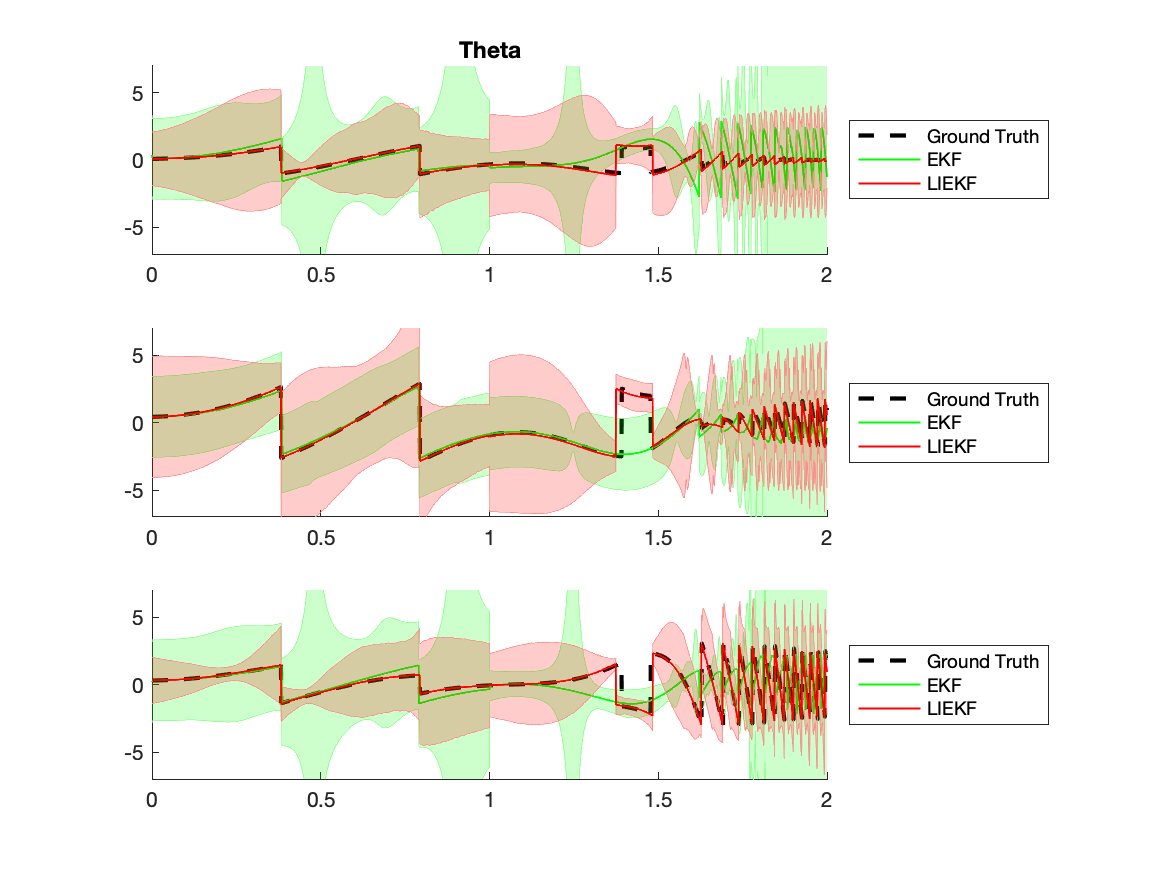
\includegraphics[width=0.45\textwidth]{sections/figures/fake_data_theta_noise.png}
    \caption{(Simulated data, measurements with noise) EKF (solid green) and LIEKF (solid red) closely follows ground truth rotation despite noisy acclerometer readings. Quantity plotted is $\theta = \mathrm{Log}(R)$, where $R$ is the rotation of the body. The covariance of each filter is shown as the shaded zone}
    \label{fig:fake_data_ang_noise}
\end{figure}

The plots in Figs.~(\ref{fig:fake_data_pos_noise},\ref{fig:fake_data_ang_noise}) show another simulated run but with some large noise added to the measurements.  In this test, we add normally disturbed, zero mean random noise with a standard deviation of 6$g$'s (58.86 m/s$^2$) to the accelerometer measurements.  Additionally we added similarly distributed noise with a standard deviation of 1 rad (57 deg) to the gyro measurements.  Initial conditions were set the ground truth and the filter was run with an update frequency of 10 Hz.  Despite the noisy conditions and the slow update rate, the filter tracked closely in position and orientation. However, there is visible disparity between the LI-EKF estimation and ground truth for velocity, especially along z-axis.  The orientation also shows less accuracy, and there is a small but noticeable steady state error in the estimation.  On another hand, the variance of the estimation is still bounded well and is not influenced much by the addition of noise.



%%%%%%%%%%%%%%%%%%%%%%%%%%%%%%%%%%%%%%%%
\subsection{Tests on Zurich Urban}
We selected the Zurich Urban data set \cite{majdik2017zurich} to test our Left-invariant EKF implementation. The data set includes GPS, accelerometer, and gyroscope measurements for a quad-rotor traversing the streets of Zurich. Additionally, the data set includes "ground-truth" data obtained using image processing. In our tests we use this estimate as our ground-truth. Using the accelerometer and gyroscope readings as our prediction step and the GPS measurements to update our prediction. The accelerometer and gyroscope update at roughly the same time step and so we assume these happen synchronously. The IMU and gyro update roughly 10 times per second. However, the GPS updates asynchronously, updating roughly once per second. To handles this, our filter runs a prediction step when it receives new IMU/gyro data and runs the correction step whenever GPS readings are received. Figures \ref{fig:Zurich_3D} and \ref{fig:Zurich_XYZ} show the results of applying our filter to the data set.

\begin{figure}
    \centering
    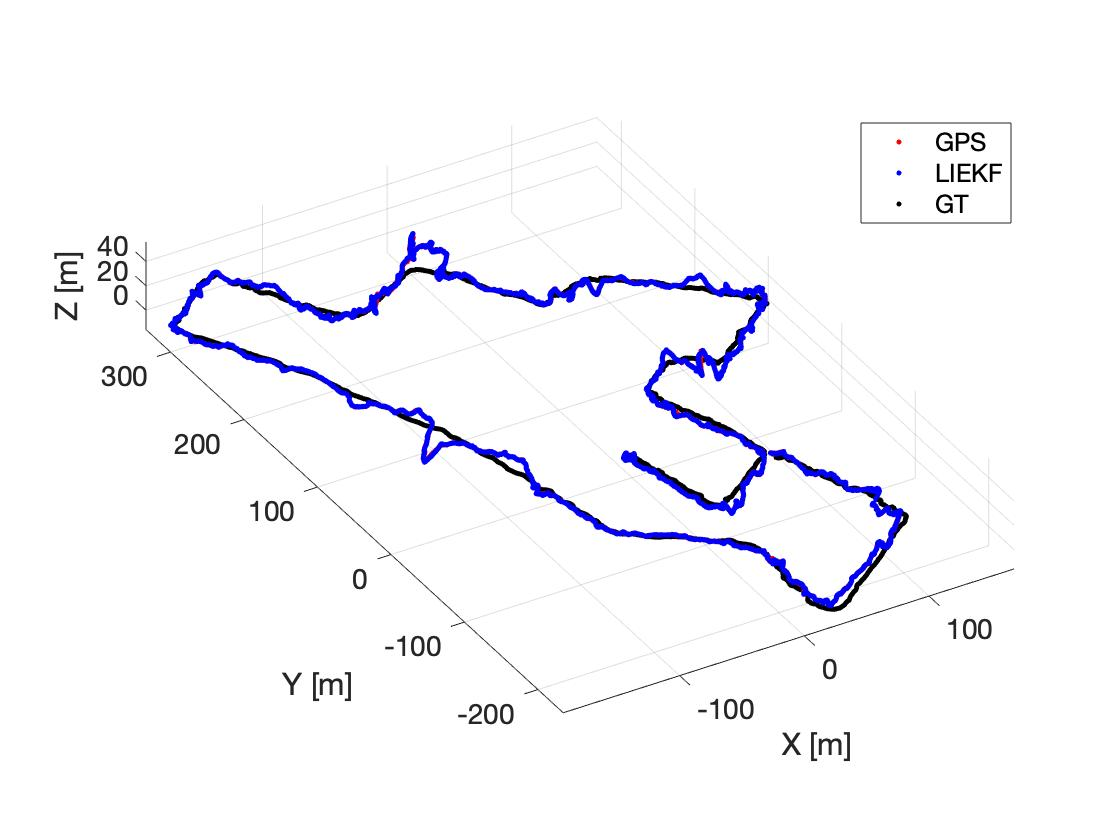
\includegraphics[width=0.45\textwidth]{sections/figures/Zurich_3D.jpg}
    \caption{The filter's state estimation on the Zurich Urban data set (blue) vs the ground truth (black). The filter follows the XY position very well, but the Z position is very noisy. The GPS readings (red) are also plotted, but are difficult to see as the estimate overlaps it in most places.}
    \label{fig:Zurich_3D}
\end{figure}

\begin{figure*}[h]
    \centering
    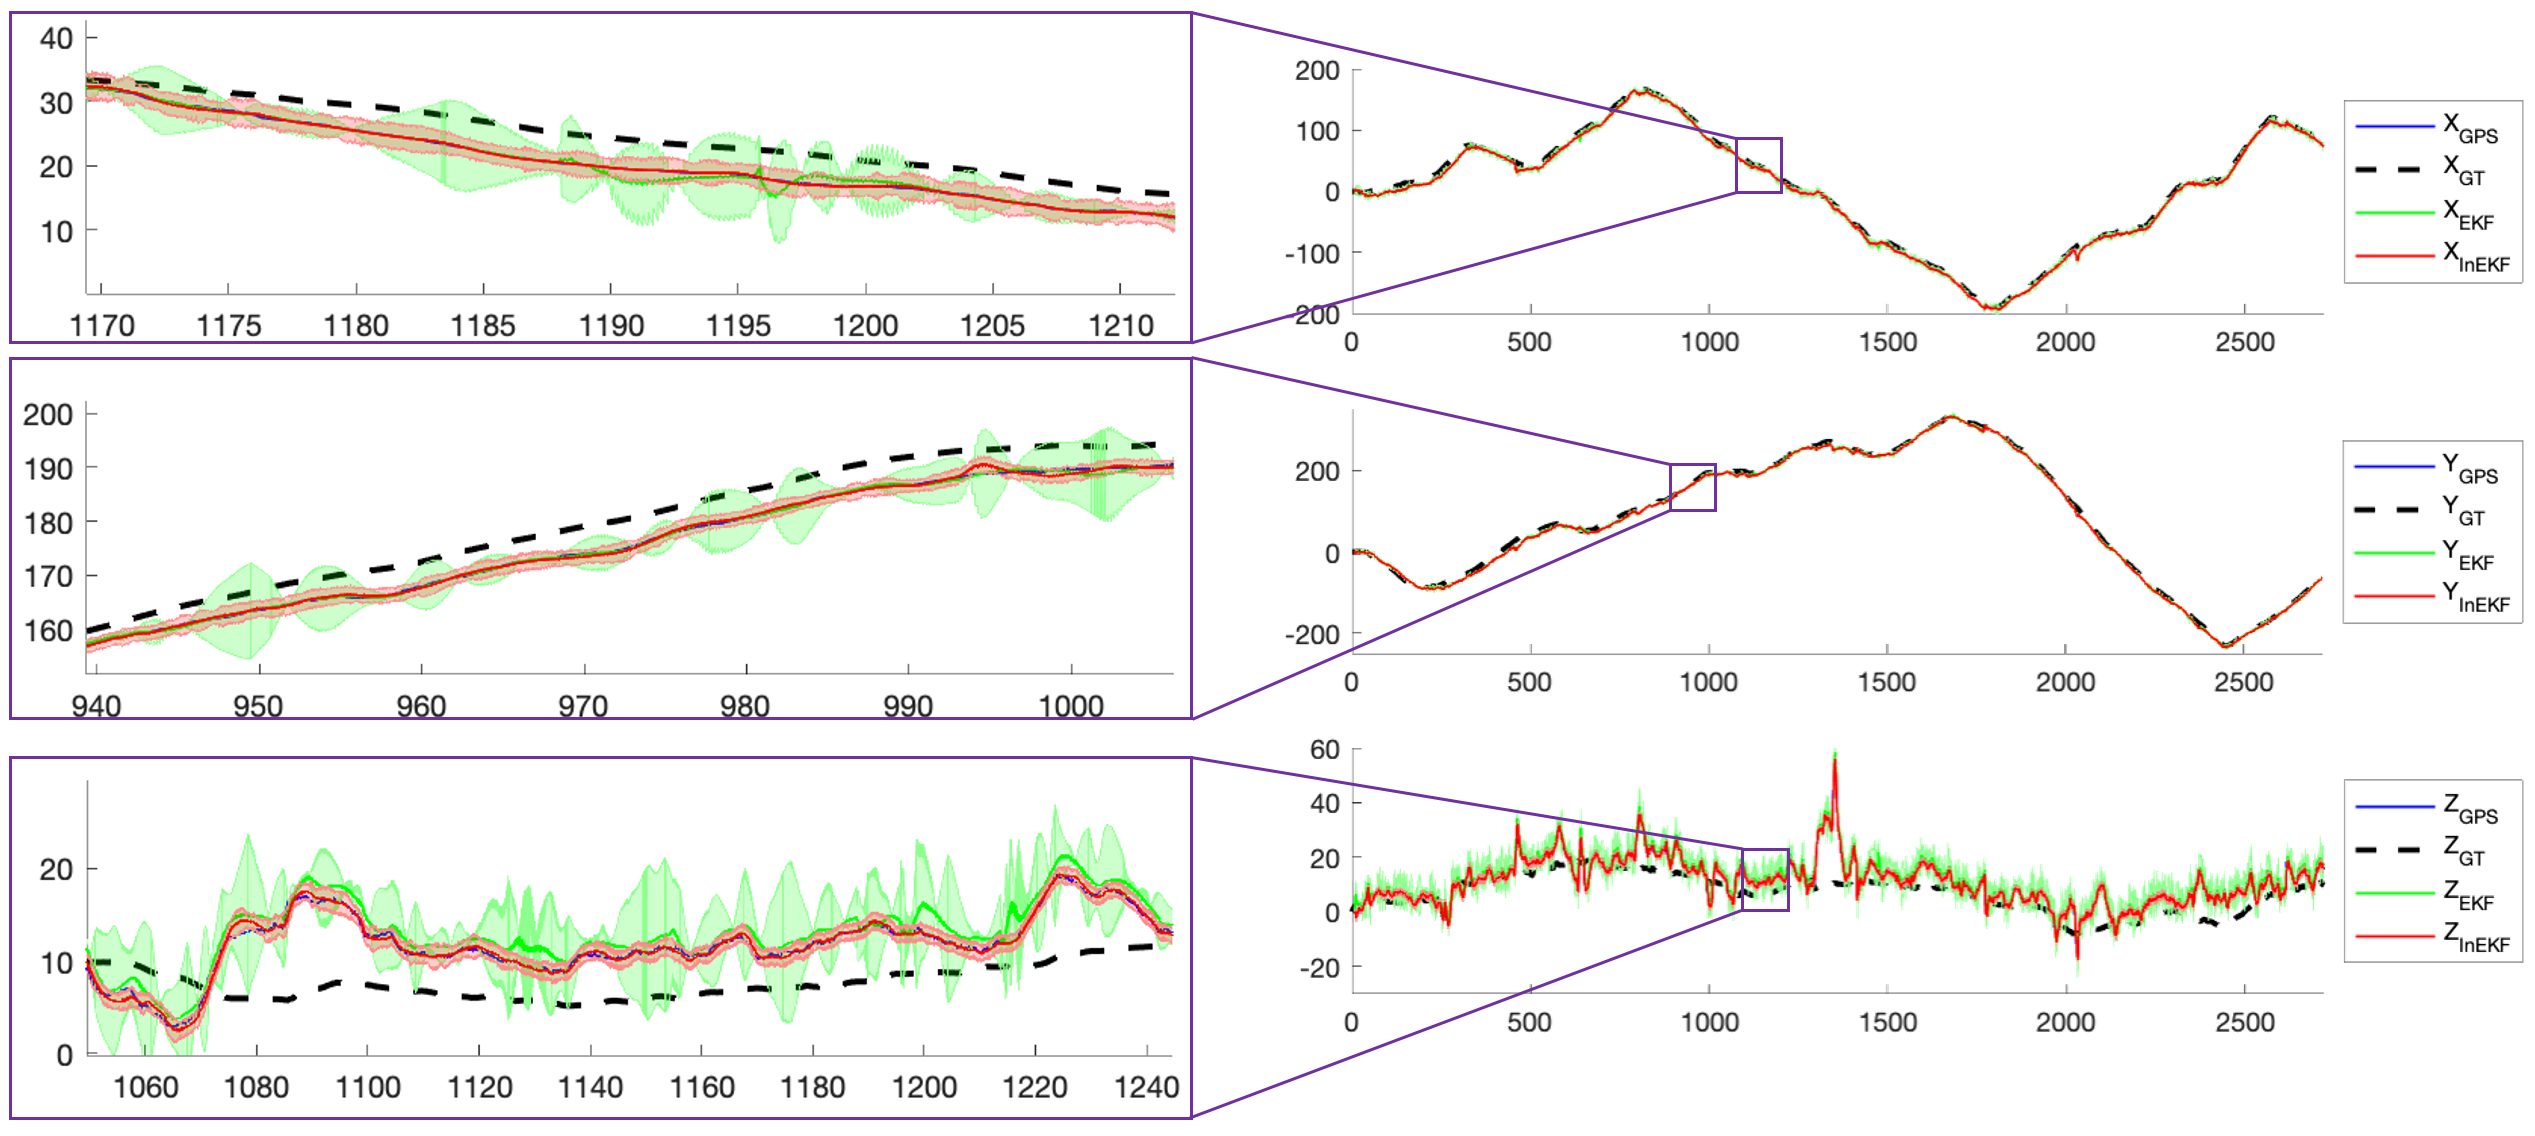
\includegraphics[width=.8\textwidth]{sections/figures/zurich_pos_std.png}
    \caption{The $x$ (top), $y$ (middle), and $z$ (bottom) positions and standard deviation of the drone over time. 
    The dashed black line is the ground truth position, and the blue line (covered by green and red) is the GPS position. The red line is the LI-EKF position and the green line is the EKF position. The shaded region is $3\sigma$ covariance. Although both trajectory follow the GPS trajectory closely, we can see that in the zoomed in version, the variance for LI-EKF is lower than the standard deviation for the EKF. This means that there is less error in the LI-EKF position}.
    \label{fig:Zurich_XYZ}
\end{figure*}

From the plots \ref{fig:Zurich_3D} and \ref{fig:Zurich_XYZ} we can see that the filter tracks the state well. However, the estimte is highly dependent upon the GPS measurements. In fact, in this case we fail to perform significantly better than just using pure GPS data. We can see in figure \ref{fig:Zurich_error} that there is some error present, but that it is nearly identical at all points to the GPS error. Even though we use a bias correction on the IMU and gyro, we fail to gain any information from their inclusion. 

The reason underneath that lies in the the quality of the measurements rather than the quality of our filter, since we have tested our filter on simulated data. Therefore, we could potentially improve the estimation results by including additional measurements such as incorporating magnetometer readings or using the gravity vector to correct the heading. Alternatively, we could add a bias correction in the measurement step which could help correct the noisy GPS data.

\begin{figure}
    \centering
    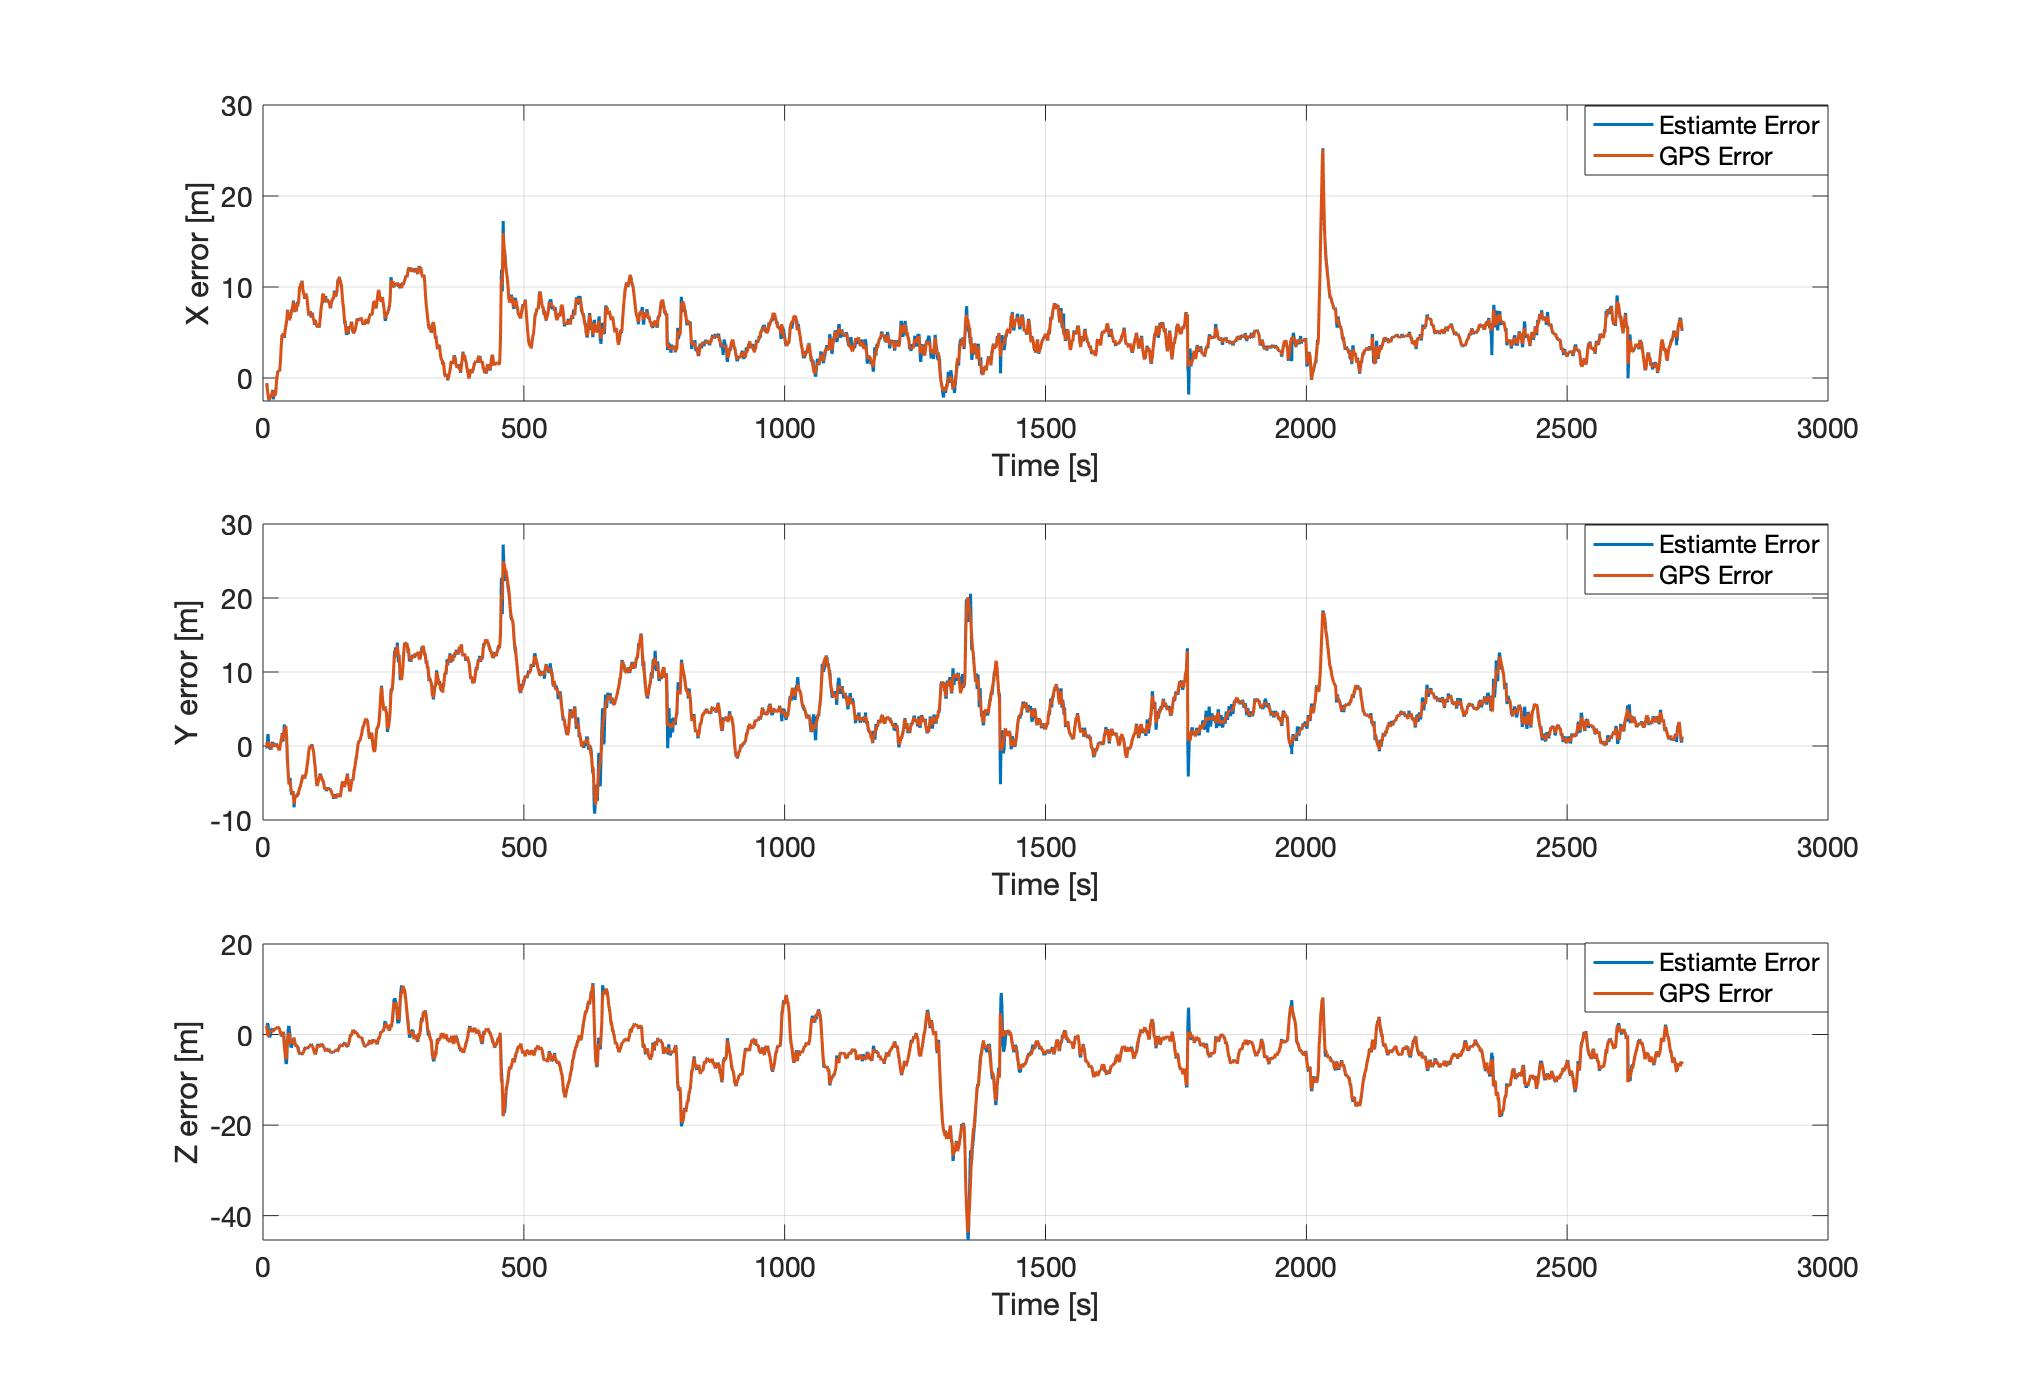
\includegraphics[width=0.45\textwidth]{sections/figures/Zurich_error.jpg}
    \caption{The X (top), Y (middle), and Z (bottom) error of the drone position over time. The LI-EKF filter error is in blue and the GPS error is in orange dashed lines. In most places these lines overlap.}
    \label{fig:Zurich_error}
\end{figure}

%%%%%%%%%%%%%%%%%%%%%%%%%%%%%%%%%%%%%%%%

\subsection{Comparison to Traditional EKF}
 As a baseline for comparison, we have developed traditional EKF algorithm in Matlab. The estimated states of the vehicle are position $\mathbf{p}(t)$, velocity $\mathbf{v}(t)$ and orientation in Euler angles $\mathbf{\phi}(t)$.

It could be observed from Figure \ref{fig:fake_data_pos} to Figure \ref{fig:fake_data_ang_noise}, with or without noise in the measurement, LI-EKF would be able to track both the position and orientation of the body accurately. In comparison, EKF magnifies local oscillation for orientation tracking, and fails to follow the ground truth position at the end when the gradient becomes steep and the nonlinearity is accumulated more, since the approximation of linearization is breached. However, the variance of LI-EKF is bounded along the trajectory because of the autonomous error dynamic of Lie algebra; however, that of EKF would grow unbounded after a short while, which also demonstrate the failing in its tracking. The inclusion of noise seems to have a small but non-critical impact on the performance of both filters, with slightly increased values of error in position and orientation tracking.

For the Zurich Urban Dataset, the advantage of LI-EKF is not obvious through visual inspection. For both of the filers, the estimation results closely follow GPS data along the trajectory, indicating the prediction from IMU is not included in the estimation process. In Figure \ref{fig:Zurich_XYZ}, it could be observed that though the estimation of the position for the two filters overlapped, the variance for LI-EKF is better bounded compared with EKF, suggesting a more reliable estimation statistically.

\section{C++ Implementation}
In addition to the Matlab scripts, we provide a C++ implementation of the filter that is capable of running on a real system.  The implementation uses the Eigen library, which is a header only library for linear algebra.  Dependency and build information is listed on our Github\footnote{\href{https://github.com/ghaggin/invariant-ekf}{https://github.com/ghaggin/invariant-ekf}}, along with usage instructions.

We verify the correctness of this implementation using an extensive testing suite.  Aside from simple checks on assumptions and basic input output, we compare the output of the filter in a number of conditions against the Matlab implementation.  For each of these test, we generate a combination of IMU and GPS measurements, and create an expected output from our Matlab filter.  Then, we run the C++ filter and compare the output to what was generated in Matlab.

We also provide an example driver for the Zurich urban dataset, where red-black trees are used to order asynchronous measurements.



\section{Conclusion}
In this project, we have developed a LI-EKF for drone localization in MATLAB and C++, taking in IMU measurement for prediction and GPS data for an update. The estimation is verified with self-generated simulated data and Zurich Urban Dataset. EKF algorithm is implemented as a baseline. For the simulated data, the LI-EKF has outperformed EKF in both tracking and boundness of variance; however, the performance of the filters are similar for the Zurich Urban Dataset, since the estimation are following GPS mostly due to the corruption of IMU data. In the future, the LI-EKF might be tested with the inclusion of more sensors or switch to another Dataset.

%
\bibliographystyle{unsrt}
\bibliography{references}
%

\begin{appendices}\label{appendices}

\section{Derivation of Discrete Dynamics} \label{sec:dyn_sec}
The continuous time differential equations which govern the motion of the rigid body are
\begin{align}
    \frac{d}{dt}\mat{R} &= \mat{R}[\mat{\omega}]_\times \label{eqn:dyn1}\\
    \frac{d}{dt}\mat{v} &= \mat{R}\mat{a} + \mat{g} \label{eqn:dyn2}\\
    \frac{d}{dt}\mat{p} &= \mat{v} \label{eqn:dyn3}
\end{align}
where $\mat{R}$ is the rotation of the body with respect to the world frame on SO(3), $\mat{\omega}$ is the angular velocity of the body frame with respect to the world frame, $\mat{v}$ is the linear velocity, $\mat{a}$ is the acceleration measured in the body frame, $\mat{g}$ is the local gravity, and $\mat{p}$ is the position of the vehicle.

The imu measurements occur in discrete increments and the time between measurements is denoted $\Delta t$. Since we have no knowledge of the acceleration and the angular rate between measurements, we are unable to exactly integrate the continuous time dynamics.  To make the problem tractable, we assume that the acceleration and rates are constant between measurements, and take the last measured value throughout the time period $\Delta t$.  Under this assumption, we can derive a exact state transition equations for $\mat{R}$, $\mat{p}$, and $\mat{v}$ between measurements using Eqns.~(\ref{eqn:dyn1})-(\ref{eqn:dyn3}).

One might be tempted to directly integrate Eqn.~(\ref{eqn:dyn2}) under the assumption of a constant $\mat{R}$.  This assumption is not valid since from Eqn.~(\ref{eqn:dyn1}), we can see that $\mat{R}$ is in fact time varying with a constant $\mat{\omega}$.  The following derivation takes the time varying nature of $\mat{R}$ into account when integrating Eqn.~(\ref{eqn:dyn2}).

We can first note that the solution to Eqn.~(\ref{eqn:dyn1}) is simply the matrix exponential function, since $[\mat{\omega}]_\times$ is a constant matrix.
\begin{align}
    \mat{R}(t) = \mat{R}_0\exp([\mat{\omega}]_\times t) \label{eqn:R_sol})
\end{align}
Using the Rodriguez rotation formula, we can rewrite Eqn.~(\ref{eqn:R_sol}) in a format that will be easier to integrate in the other dynamics equations.
\begin{align}
    \mat{R}(t) &= \mat{R}_0 \left[\mat{I} + \frac{\sin(\Vert\mat{\omega} t\Vert)}{\Vert\mat{\omega}\Vert}[\mat{\omega}]_\times + \frac{1 - \cos(\Vert\mat{\omega} t\Vert)}{\Vert\mat{\omega}\Vert^2}[\mat{\omega}]_\times^2\right] \nonumber\\
    &= R_0 \mat{\Gamma}_0(t)
\end{align}
Here we denote the bracketed expression as $\mat{\Gamma}_0 (t)$ and notice that all matrices are constants multiplied by scalar trigonometric functions.

Now, writing the velocity dynamics in terms of $R(t)$, we get
\begin{align}
    \frac{d}{dt} v &= \mat{R}(t)\mat{a} + \mat{g} \\
    \frac{d}{dt} v &= \mat{R}_0\mat{\Gamma}_0(t)\mat{a} + \mat{g}
\end{align}
Integrating this with respect to time, we find
\begin{align}
    \mat{v}(t) = R_0 \left(\int \mat{\Gamma}_0(t) dt\right) + \mat{g}t + C_1 \label{eqn:v_indef}
\end{align}
where
\begin{multline}
    \int\mat{\Gamma}_0(t) dt =\\\mat{I}t + \frac{-\cos(\Vert\mat{\omega} t\Vert)}{\Vert\mat{\omega}\Vert^2}[\mat{\omega}]_\times + \frac{\Vert\mat{\omega} t\Vert - \sin(\Vert\mat{\omega} t\Vert)}{\Vert\mat{\omega} \Vert^3}[\mat{\omega}]_\times{}^2
\end{multline}
Solving for C in Eqn.~(\ref{eqn:v_indef}),
\begin{align}
    \mat{v}(0) = \mat{v}_0 = -\frac{[\mat{\omega}]_\times}{\Vert\mat{\omega}\Vert^2} + C_1
\end{align}
And plugging this into (\ref{eqn:v_indef}),
\begin{align}
    \mat{v}(t) = \mat{R}_0\mat{\Gamma}_1(t)\mat{a}t + \mat{g}t + \mat{v}_0
\end{align}
with
\begin{align}
    \mat{\Gamma}_1(t)t = \mat{I}t + &\frac{1-\cos(\Vert\mat{\omega t}\Vert)}{\Vert\mat{\omega }\Vert^2}[\mat{\omega} ]_\times + \frac{\Vert\mat{\omega}\Vert - \sin(\Vert\mat{\omega t} \Vert)}{\Vert\mat{\omega}\Vert^3}[\mat{\omega}]_\times{}^2
\end{align}
Note that we specify $\mat{\Gamma}_1(t) t$, which is $\mat{\Gamma}_1$ as a function of $t$ times the variable $t$.  We use this expression so that the next integral is clearer.  In the paper, we remove the factor of $t$ from the function to make the equation clearer and in terms of $\mat{\omega} t$ as a unit.

Now we can integrate the position dynamics.
\begin{align}
    \frac{d}{dt}\mat{p} &= \mat{R}_0\mat{\Gamma}_1(t)\mat{a}t + \mat{g}t + \mat{v}_0 \\
    \mat{p} &= \mat{R}_0 \left(\int \mat{\Gamma}_1(t)t\ dt\right)\mat{a} + \frac{1}{2}\mat{g}t^2 + \mat{v}_0t + C_2 \label{eqn:p_indef}
\end{align}
where
\begin{multline}
    \int \mat{\Gamma}_1(t)t\ dt =
    \frac{1}{2}\mat{I}t^2 + \frac{\Vert\mat{\omega} t\Vert - \sin(\Vert\mat{\omega} t\Vert)}{\Vert\mat{\omega}\Vert^3}[\mat{\omega}]_\times +\\ \frac{\Vert\mat{\omega} t\Vert^2 + 2\cos(\Vert\mat{\omega} t\Vert)}{2\Vert\mat{\omega}\Vert^4}[\mat{\omega} ]_\times{}^2
\end{multline}
Solving for $C_2$ in (\ref{eqn:p_indef}),
\begin{align}
    \mat{p}(0) = \mat{p}_0 = \frac{[w]_\times^2}{\Vert w\Vert^4}+C_2
\end{align}
and plugging this back into (\ref{eqn:p_indef}),
\begin{align}
    \mat{p}(t) = \mat{R}_0\mat{\Gamma}_2(t)\mat{a}t^2 + \frac{1}{2}\mat{g}t^2 + \mat{v}_0t + \mat{p}_0
\end{align}
with
\begin{multline}
    \mat{\Gamma}_2(t) = \frac{1}{2}\mat{I} + \frac{\Vert\mat{\omega} t\Vert - \sin(\Vert\mat{\omega} t\Vert)}{\Vert\mat{\omega} t\Vert^3}[\mat{\omega} t]_\times +\\ \frac{\Vert\mat{\omega} t\Vert^2 + 2\cos(\Vert\mat{\omega} t\Vert) - 2}{2\Vert\mat{\omega} t\Vert^4}[\mat{\omega} t]_\times{}^2
\end{multline}

Thus, if we take the initial conditions to be at timestep $k$ and the value at $k+1$ to be the quantity of the state transition over time $\Delta t$, the discrete dynamical equations become
\begin{align}
    \mat{R}_{k+1} &= \mat{R}_{k}\exp([\mat{\omega}]_\times \Delta t) \\
    \mat{v}_{k+1} &= \mat{R}_k \mat{\Gamma}_1(\mat{\omega} \Delta t) \mat{a} \Delta t + \mat{g} \Delta t + \mat{v}_k \\
    \mat{p}_{k+1} &= \mat{R}_k \mat{\Gamma}_2(\mat{\omega} \Delta t) \mat{a} \Delta t^2 + \frac{1}{2}\mat{g}  \Delta t^2 + \mat{v}_k \Delta t + \mat{p}_k
\end{align}

\section{Simulated Data} \label{sec:fake_data}
The simulated data used for the tests shown in Sec.~(\ref{sec:simulation_results}) is listed here.  Each dimension of the angle or positional data is created from a randomly generated polynomial, where each coefficient is sampled from some random distribution.  Each polynomial is a 4th order polynomial and can be evaluated at any point in time.  The coefficients are listed in Tabs.~(\ref{tab:pos_coef}, \ref{tab:ang_coef}), with the first coefficient listed being the scalar multiplied by $x^4$ and the last being the constant ($x^0$ term).  This the default ordering that the Matlab function \texttt{polyval} expects. 

\begin{table}[h]
    \centering
    \caption{Position ground truth random polynomial coefficients.}
    \begin{tabular}{cl}
        $x$: & \texttt{[13.862459 -16.814181 0.209844 -17.388540 -2.875107]} \\
        $y$: & \texttt{[-16.138763 -14.913601 3.869812 -10.959520 -15.722173]}\\
        $z$: & \texttt{[-11.187752 -6.006949 -1.288501 -11.930271 5.616269]}
    \end{tabular}
    \label{tab:pos_coef}
\end{table}

\begin{table}[h]
    \centering
    \caption{Angle ground truth random polynomial coefficients.}
    \begin{tabular}{cl}
        $x$: & \texttt{[-0.677207 0.209469 -4.524294 11.745498 3.200167]} \\
        $y$: & \texttt{[-13.508056 8.030094 18.582043 0.000334 15.580803]}\\
        $z$: & \texttt{[-6.335454 2.685765 -2.898161 -2.530109 11.062367]}
    \end{tabular}
    \label{tab:ang_coef}
\end{table}

\end{appendices}

\end{document}

